 \documentclass[a4paper,12pt]{report}

\usepackage{alltt, fancyvrb, url}
\usepackage{graphicx}
\usepackage[utf8]{inputenc}
\usepackage{float}
\usepackage{hyperref}
\usepackage{xcolor}
\usepackage{listings}

% Questo commentalo se vuoi scrivere in inglese.
\usepackage[italian]{babel}

\usepackage[italian]{cleveref}

\lstset{ %
   backgroundcolor=\color{white},   % choose the background color
   basicstyle=\footnotesize\ttfamily,        % the size of the fonts that are used for the code
   breakatwhitespace=false,         % sets if automatic breaks should only happen at whitespace
   breaklines=true,                 % sets automatic line breaking
   captionpos=t,                    % sets the caption-position to bottom
   commentstyle=\color{mygreen},    % comment style
   %deletekeywords={...},            % if you want to delete keywords from the given language
   %escapeinside={\%*}{*)},          % if you want to add LaTeX within your code
   frame=single,                    % adds a frame around the code
   keepspaces=true,                 % keeps spaces in text, useful for keeping indentation of code (possibly needs columns=flexible)
   keywordstyle=\color{blue},       % keyword style
   language=java,                   % the language of the code
   morekeywords={var},            % if you want to add more keywords to the set
   numbers=left,                    % where to put the line-numbers; possible values are (none,left, right)
   numbersep=5pt,                   % how far the line-numbers are from the code
   numberstyle=\tiny\color{gray}, % the style that is used for the line-numbers
   rulecolor=\color{black},         % if not set, the frame-color may be changed on line-breaks within not-black text (e.g. comments (green here))
   showspaces=false,                % show spaces everywhere adding particular underscores; it overrides 'showstringspaces'
   showstringspaces=false,          % underline spaces within strings only
   showtabs=false,                  % show tabs within strings adding particular underscores
   stepnumber=1,                    % the step between two line-numbers. If it's 1, each line will be numbered
   stringstyle=\color{mymauve},     % string literal style
   tabsize=2,                       % sets default tabsize to 2 spaces
   %title=\lstname                   % show the filename of files included with \lstinputlisting;
 %also try caption instead of title
 %  literate={à}{{\`a}}1
 %      {è}{{\`e}}1
 %      {ò}{{\`o}}1
 %      {ì}{{\`i}}1
 %      {ù}{{\`u}}1
}

\title{Relazione per\\``Programmazione ad Oggetti''\\Stubborn}

\author{Mario Ciccioni, Andrea Bianchi}
\date{\today}


\begin{document}

\maketitle

\tableofcontents

\chapter{Analisi}

Il software, un videogioco 2D bird-eye view survival, proporra' al videogiocatore un'esperienza di un classico videogame survival dove lo scopo e' quello di resistere il maggior tempo possibile cercando anche di accumulare punti durante la partita.
Il videogiocatore avra' la possibilita' di muoversi nel mondo di gioco con il suo personaggio, sopravvivere ai nemici che incontrera' nella mappa, raccogliere oggetti e recuperare vita.
Per bird-eye view si intende una visuale dall'alto del mondo di gioco, similare a quella di titoli già esistenti come i vecchi giochi di Legend Of Zelda per NES.

\section{Requisiti}

\subsubsection{Requisiti funzionali}
\begin{itemize}
	\item Una volta avviato il software verra' presentato a schermo un menu' di gioco dove il videogiocatore potra' scegliere se iniziare una nuova partita, visualizzare la classifica dei punteggi o uscire dall'applicazione.
    \item La partita termina solo quando il personaggio perdera' tutte le vite a sua disposizione.
\end{itemize}

\subsubsection{Requisiti non funzionali}
\begin{itemize}
	\item Stubborn dovra' garantire una buona gestione delle risorse, mantenere una buona prestazione per evitare di rovinare l'esperienza di gioco e una grafica che permetta il chiaro riconoscimento di oggetti di gioco e nemici sparsi per la mappa.
    \item Tutte le informazioni relative alla partita in corso saranno mostrate a schermo in modo intuitivo, senza essere troppo invasive ma allo stesso tempo facilmente controllabili anche durante la partita.
\end{itemize}

% DA AGGIUNGERE: USEREMO LA PAROLA CONTROLLER AL POSTO DI PRESENTER PERCHE' PIU ESPLICATIVA E VICINO ALLA LETTERATURA ANCHE SE IN REALTA' IL MODO PRECISO DI CHIAMARLO IN MVP E' PRESENTER 
\section{Analisi e modello del dominio}
Il videogioco denominato Stubborn proporra' al giocatore delle semplici sfide, alcune di esse saranno implementate mentre altre potranno essere aggiunte in futuro.
In particolare il giocatore avra' la possibilita' di raccogliere oggetti collezionabili che si trovano sulla mappa fin dall'inizio della partita ed al tempo stesso non deve prendere danno dai nemici.
Il player ha a disposizione 3 vite, se verra' colpito da un nemico ne perdera' una.
La fine del gioco avverra' solo quando il player finira' le vite a sua disposizione.
Riguardo ai nemici, essi verranno spawnati nella mappa di gioco con una logica random, a inizio partita, mentre per quanto riguarda la loro Ai puo' essere random oppure focalizzata sull'inseguimento del player.
Alcune funzionalita' come diverse implementazioni di Ai nemici, attacco player > nemici, gameover ecc. verranno implementate in futuro e quindi il software sara' progettato in modo da appliare lo stesso in un futuro in modo semplice e veloce.
Di seguito viene mostrato lo schema UML dell'anali del problema contenenete le entita' principali che costutuiscono il problema \Cref{img:analysisUML}.

\begin{figure}[H]
\centering{}
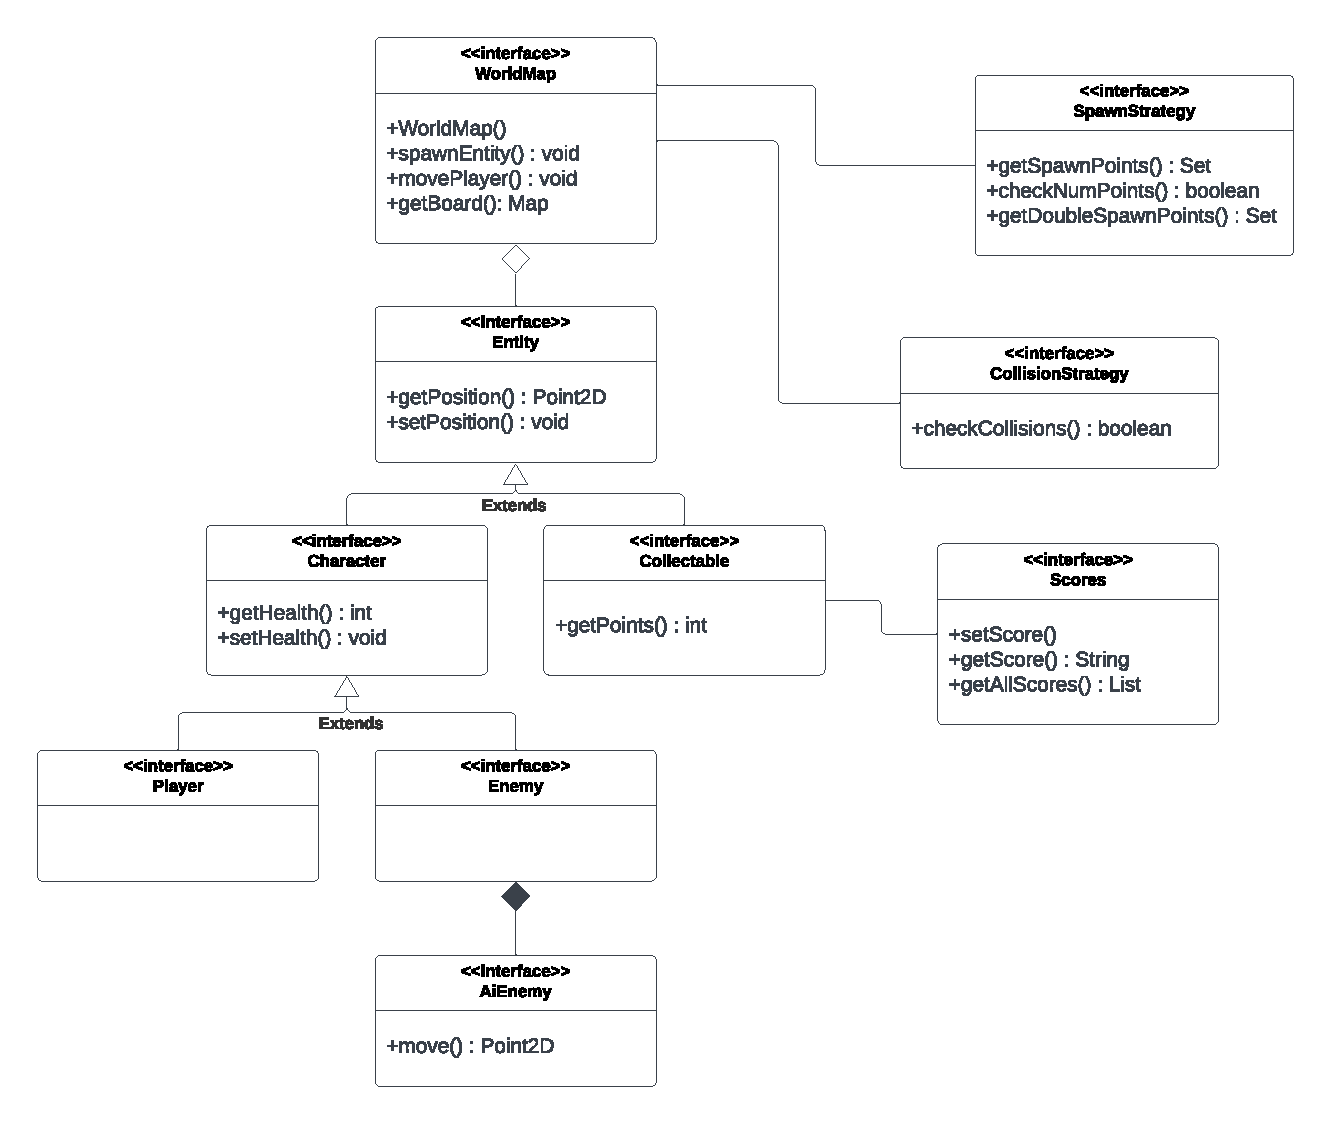
\includegraphics[width=\textwidth,height=\textheight,keepaspectratio]{img/analysisUML.pdf}
\caption{Schema UML dell'analisi del problema, con rappresentate le entità principali ed i rapporti fra loro}
\label{img:analysisUML}
\end{figure}

\chapter{Design}

\section{Architettura}
Premessa: utilizzeremo il termine Controller al posto di Presenter (come si chiama effettivamente nel pattern MVP) perche' piu' esplicativo e vicino alla letteratura.

Il pattern architetturale scelto per la realizzazione del software e' MVP (Model View Presenter). In particolare abbiamo adottato la variante MVP Passive View, ossia la view e' un componente completamente passivo del sistema e non svolge nessuna operazione ma viene solo aggiornata dai Controller.
L'entry point del model e' WorldMap, essa e' la main class del software che contiene la logica generale del videogioco. Per quanto riguarda i Controller abbiamo deciso di adottare una logica di divisione dello stesso. Per ogni macro compito del software abbiamo implementato un suo specifico Controller in grado di comunicare con la view e se necessario comunicare con/modificare lo stato del model.
I principali vantagggi dell'adottare questa architettura sono i seguenti:
\begin{itemize}
	\item Fornire al software una maggiore modularita', offrendo la possibilita' di rendere indipendenti gli elementi visivi, di model e di controller. 
    \item E' possibile cambiare libreria grafica senza che essa impatti sul Controller, ne tantomeno sul Model (la logica del sistema non risentira' in alcun modo di questi cambiamenti). In quando e' possibile incapsulare la logica di view rendendo possibile l'integrazione di una nuova libreria grafica senza interferire con l'architettura del software.
    \item Offre una semplice gestione tri i vari Controller, permettendo una modularita' nella gestione degli stessi.
    \item Con l'aggiunta di nuove funzionalita', essere risultano molto piu' facili da testare in quanto la maggior parte del flusso di esecuzione e' gestito dai Controller.
\end{itemize}
% schema UML generale di interazione tra Controller e Model

\section{Design dettagliato}
\textbf{ANDREA BIANCHI}
\\ \\
\textit{Generazione/Posizionamento delle entità all’interno della mappa di gioco}
\begin{itemize}
    \item \textbf{Problema:} La corretta generazione del posizionamento del protagonista, dei nemici e degli oggetti raccoglibili (entità), che saranno collocati all’interno della mappa di gioco.
    \item \textbf{Soluzione:} Il sistema utilizza Pattern Strategy, rappresentato dall’ interfaccia \verb|SpawnStrategy|: questo approccio ci permette di disaccoppiare l’effettiva mappa di gioco dalle diverse possibili implementazioni e variazioni su come verranno generati i punti dove saranno collocate le entità di gioco; si offre così una grande estendibilità utile ad ulteriori implementazioni e variazioni anche più complesse, permettendo la creazioni di sottoclassi ed eliminando complessità, dato che ogni comportamento viene implementato dalla propria classe (evitiamo l’uso di statement condizionali).
\end{itemize}
\begin{figure}[H]
\centering{}
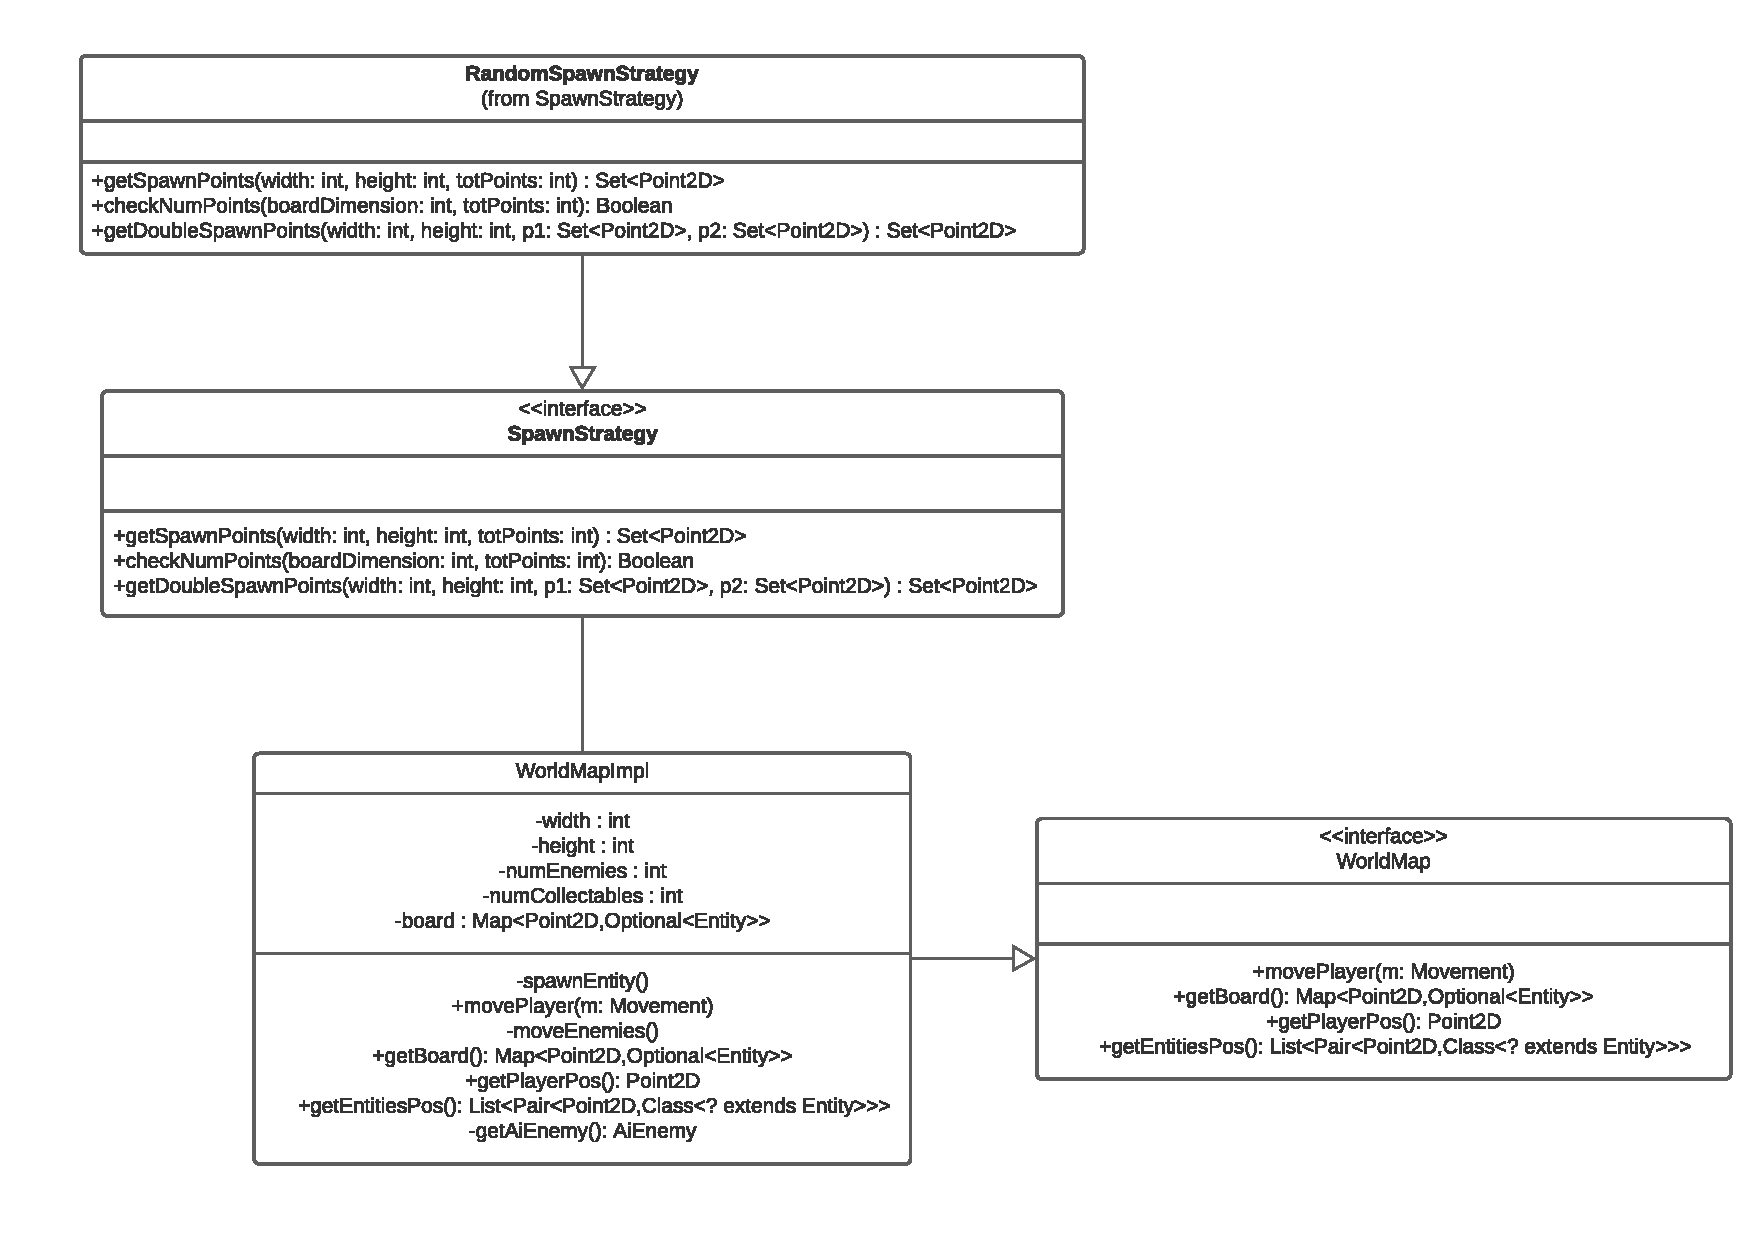
\includegraphics[width=\textwidth,height=\textheight,keepaspectratio]{img/spawnStrategy.pdf}
\caption{Schema UML a rappresentare la soluzione per la SpawnStrategy, con tanto di implmentazione RandomSpawnStrategy}
\label{img:spawnStrategyUML}
\end{figure}

\textit{Interazioni tra le varie entità e con i confini della mappa di gioco.}
\begin{itemize}
    \item \textbf{Problema:} Entità in grado di muoversi all’interno della mappa, quali il giocatore e il nemico, rischiano di riuscire a superare i confini della mappa o di raggiungere entrambi una stessa posizione, questo rende necessario lo sviluppo di un sistema di collisioni.
    \item \textbf{Soluzione:} Il sistema si avvale nuovamente del Pattern Strategy, tramite l’interfaccia \verb|CollisionStrategy|: questo sistema offre una forma di riuso di codice per gestire eventi di collisione comuni a tutte le entità, come nel caso delle interazioni di esse con i confini della mappa, permettendo anche l implementazione di estensioni personalizzate per alcune tipologie di entità, come ad esempio il fatto che due nemici o un nemico e il giocatore non potranno mai andare ad occupare la stessa cella, o che non vi sia alcun tipo di collisione tra Player e gli oggetti raccoglibili (il protagonista può andare nella cella dove si trova il collezionabile e “raccoglierlo”).
\end{itemize}
\begin{figure}[H]
\centering{}
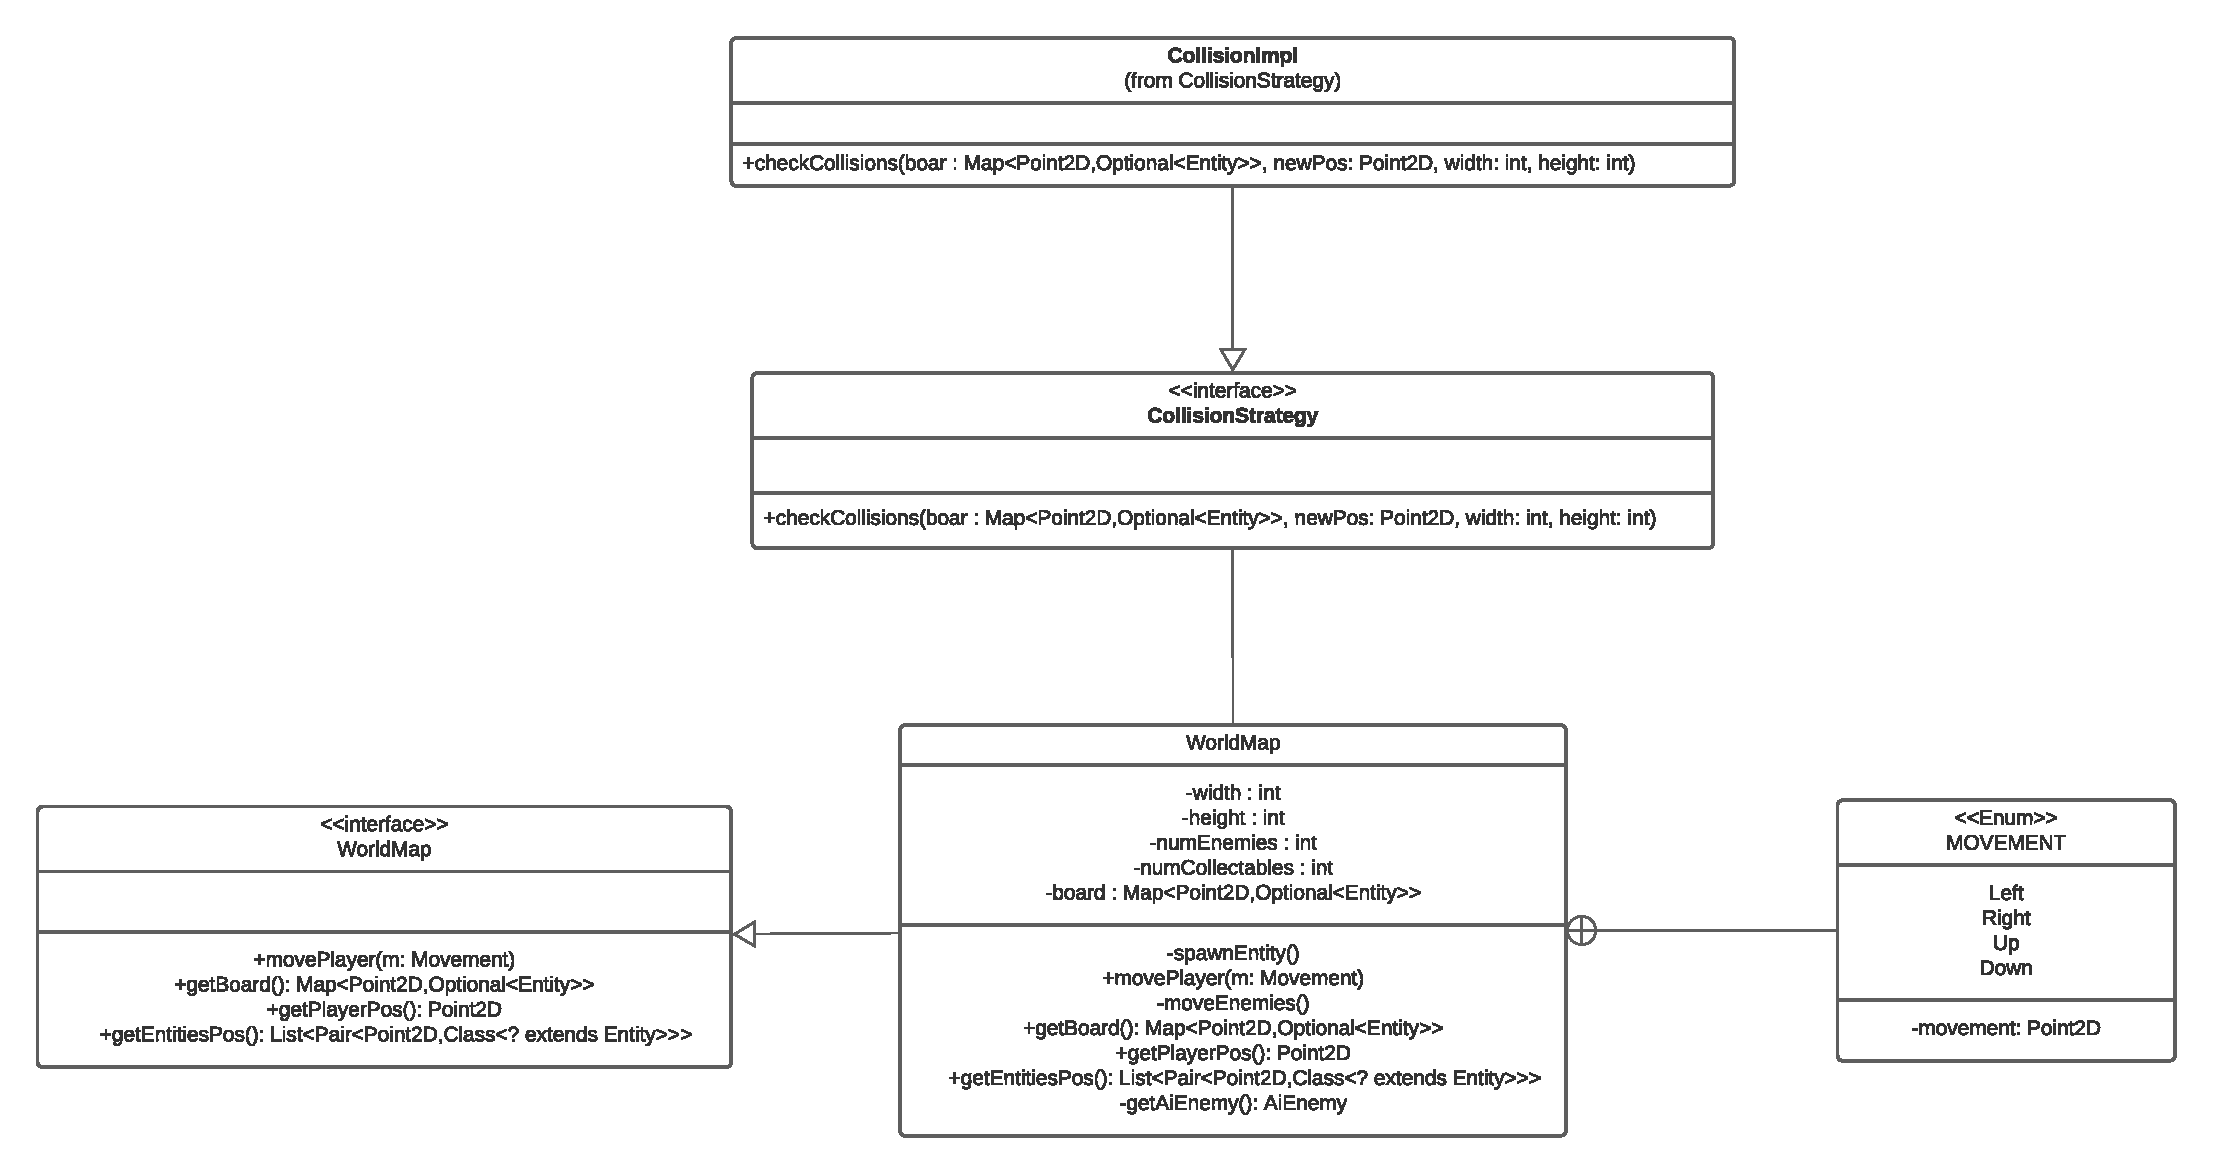
\includegraphics[width=\textwidth,height=\textheight,keepaspectratio]{img/collisionStrategy.pdf}
\caption{Schema UML a rappresentare la soluzione per la CollisionStrategy, con tanto di implmentazione CollisionStrategyImpl}
\label{img:collisionStrategyUML}
\end{figure}
% DA AGGIUNGERE GLI SCHEMI UML DEGLI SPECIFICI SOTTO SISTEMI
\textbf{MARIO CICCIONI}
\\ \\
\textit{Creazione delle entita' Player e Enemy}
\begin{itemize}
    \item \textbf{Problema:} Fin dall'inizio, durante l'analisi del progetto da realizzare, ci siamo imbattuti nel problema delle varie tipologie di entita' presenti del videogioco. Infatti era necessario creare una gerarchia di Interfacce in grado di modellare al meglio la struttura delle entita' ottimizzando al massimo il riutilizzo e l'ampliamento futuro del progetto.
    \item \textbf{Soluzione:} Le entita' che compongono il videogico sono di 3 principali tipologie: 
    \begin{itemize}
        \item \verb|Player|
        \item \verb|Enemy|
        \item \verb|Collectable|
    \end{itemize}
    A questo punto e' stato necessario creare una interfaccia chiamata \verb|Entity|, che contiene un contratto generale per tutte le tipologie di entita', a sua volta ho creato poi due interfacce che estendono da \verb|Entity| chiamate \verb|Character| e \verb|Collectable|, ed infine le due interfacce \verb|Player| e \verb|Enemy|. Le interfacce che sono poi effettivamente implementate in classi sono \verb|Collectable|, \verb|Player| e \verb|Enemy|. Questa implementazione fa uso del pattern Strategy, molto utile per tutti i vantaggi che offre dichiarati nel problema qui sopra. Di seguito lo schema UML rappresentante la gerarchia di interfacce/classi che modellano il problema. \Cref{img:EntityUML}.
    \item \textbf{Miglioramenti apportabili a questa soluzione:} La soluzione implementata e' sicuramente buona ma non ottima. Senza avere avuto le problematiche di tempo generate dall'abbandono di un membro del gruppo, con la conseguente ricaduta del suo lavoro nelle spalle dei due membri rimasti, avrei provato a programmare diversamente questo concetto di Entita' sviluppando una AbstractFactory (Design Pattern/Creational Pattern) in grado di modellare ancora meglio questo concetto generando un codice maggiormente modulabile, compatibile e modificabile.
    \begin{figure}[H]
        \centering{}
        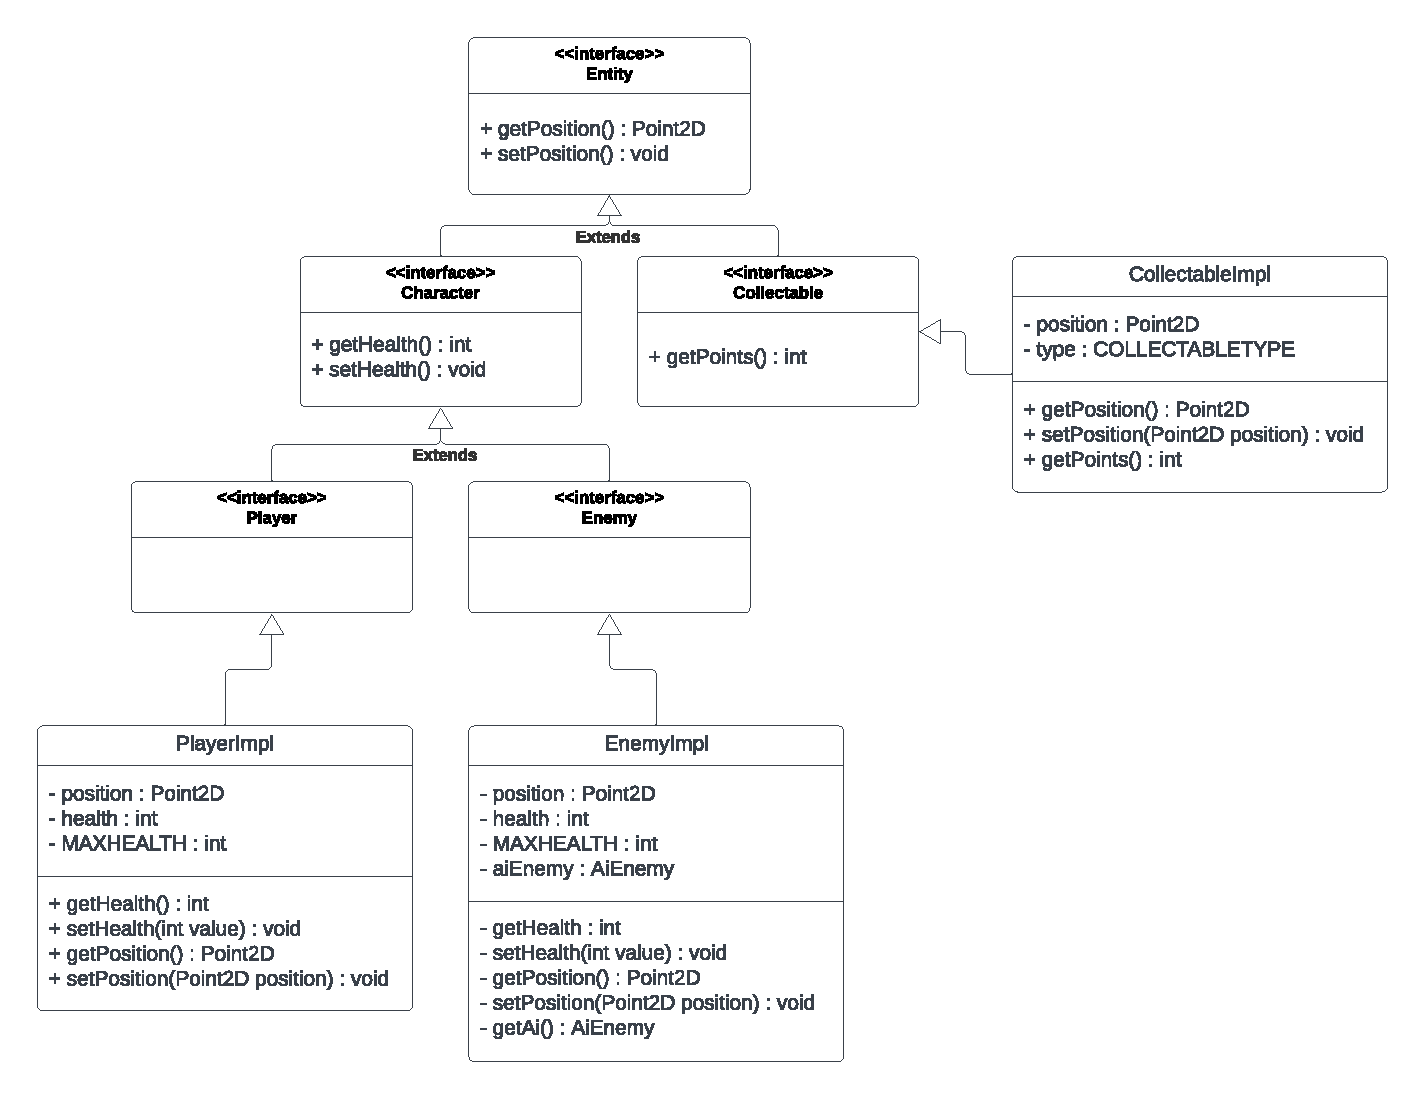
\includegraphics[width=\textwidth,height=\textheight,keepaspectratio]{img/EntityUML.pdf}
        \caption{Schema UML rappresentante la gerarchia delle classi/interfacce di Entity.}
        \label{img:EntityUML}
    \end{figure}
\end{itemize}
\textit{Implementazione dell'intelligenza artificiale dei nemici e sue varianti}
\begin{itemize}
    \item \textbf{Problema:} A differenza degli oggetti collezionabili che si trovano nella mappa di gioco e sono elementi statici, i nemici devono necessariamente possedere un'intelligenza artificiale che gli permetta di muoversi. Quindi e' stato necessario implementare un sistema di Ai in grado di soddisfare questo problema.
    \item \textbf{Soluzione:} Per risolvere in modo pulito e per sfruttare al meglio il riutilizzo di codice ho adottato l'uso del pattern Strategy, il quale e' ottimo per affrontare e risolvere al meglio questo problema. Con l'interfaccia \verb|AiEnemy| viene dichiarato il contratto che deve essere rispettato da tutte le classi che estendono da essa. Piu' in particolare ho implementato due diverse tipologie di intelligenza: \verb|RandomAiEnemy| e \verb|FocusAiEnemy|.
    \verb|RandomAiEnemy| e' un'intelligenza che fa muovere il nemico in modo completamente casuale all'interno della mappa di gioco.
    \verb|FocusAiEnemy| invece, e' un'intelligenza che offre al nemico la capacita' di inseguire il Player.
\end{itemize}
Di seguito viene mostrato lo schema UML del modello di questo specifico sotto-sistema. \Cref{img:AiEnemyUML}.
\begin{figure}[H]
     \centering{}
     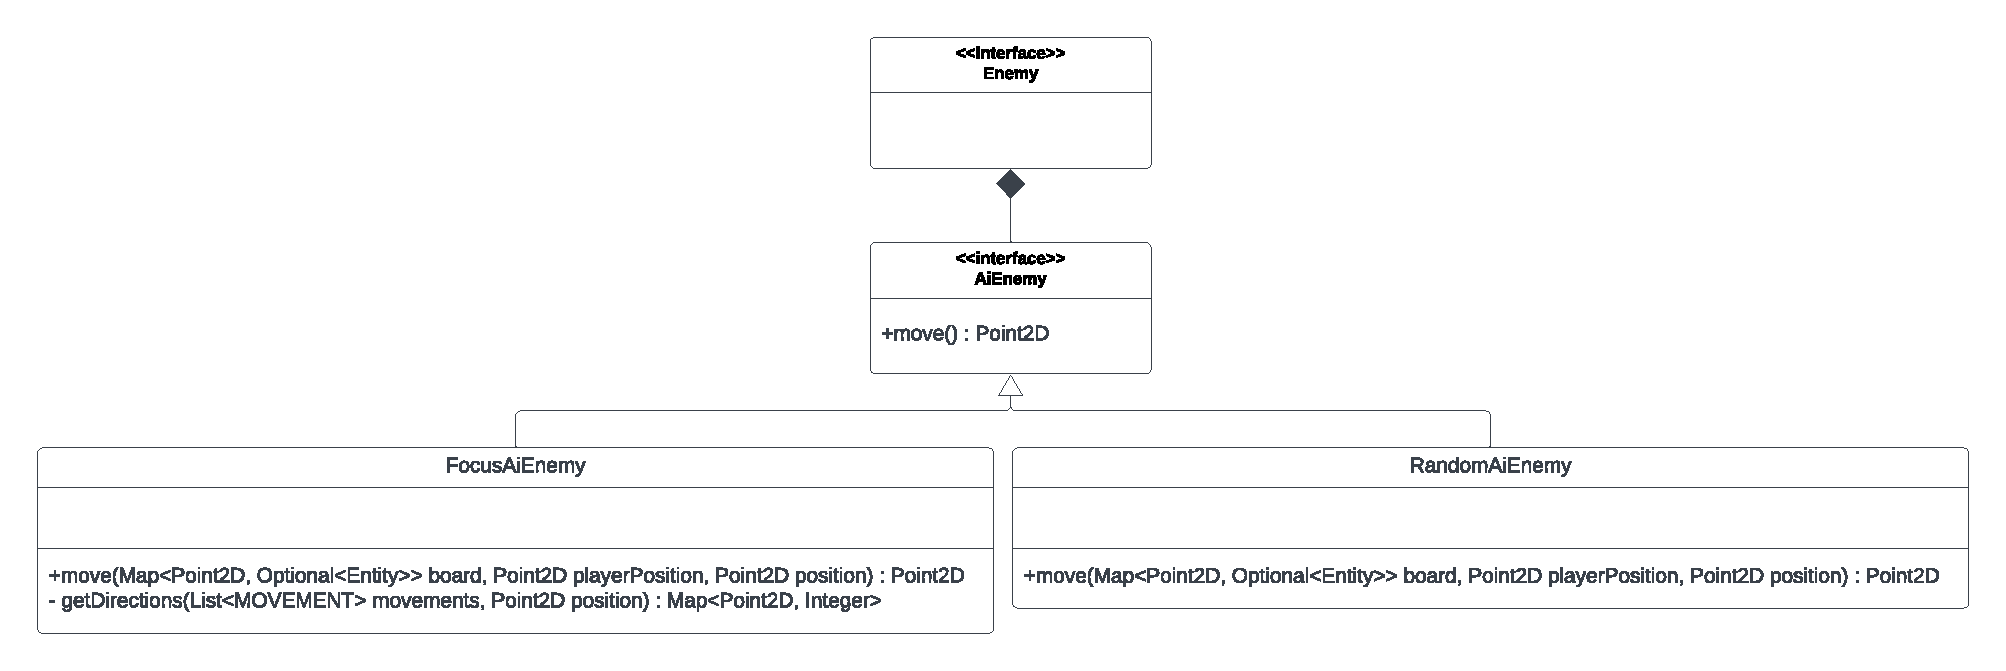
\includegraphics[width=\textwidth,height=\textheight,keepaspectratio]{img/AiEnemyUML.pdf}
     \caption{Schema UML rappresentante la gerarchia delle classi/interfacce che modellano l'intelligenza artificiale}
     \label{img:AiEnemyUML}
 \end{figure}
\textit{Gestione punteggi giocatore}
\begin{itemize}
    \item \textbf{Problema:} Per tracciare i punteggi ottenuti nelle varie partite di gioco e' stato necessario implementare un sistema di salvataggio punteggi. Con la possibilita', cosi', di essere visualizzati dall'utente a fine o inizio di una partita.
    \item \textbf{Soluzione:} Per fare cio' e' stato necessario implementare una logica di salvataggio punteggi su file e visualizzazione sull'interfaccia grafica in una sezione appositamente creata per questo scopo (voce di menu Score con visualizzazione a tabella Nome : Punteggio).
    Dal punto di vista progettuale ho utilizzato anche per risolvere questo problema il pattern strategy creando un'interfaccia \verb|Scores| e la sua implementazione \verb|ScoresImpl| offrendo cosi' facile estensione o cambiamento del codice.
\end{itemize}
Di seguito viene mostrato lo schema UML del modello di questo specifico sotto-sistema. \Cref{img:ScoresUML}.
\begin{figure}[H]
     \centering{}
     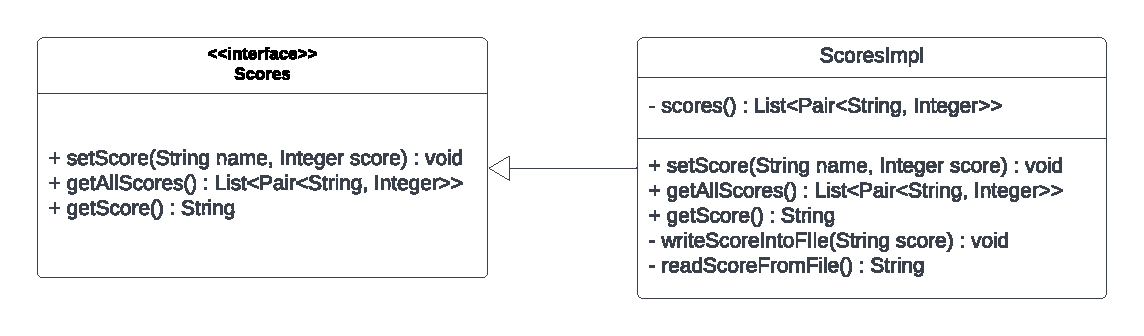
\includegraphics[width=\textwidth,height=\textheight,keepaspectratio]{img/ScoresUML.pdf}
     \caption{Schema UML rappresentante la gerarchia delle classi/interfacce che modellano il sottosistema che gestisce i punteggi partite.}
     \label{img:ScoresUML}
\end{figure}
\chapter{Sviluppo}
\section{Testing automatizzato}
Numerosi sono i compiti e i dettagli che durante lo sviluppo del progetto si sono dovuti in particolare modo controllare e testare affinchè l'applicazione funzionasse correttamente. Per elaborare ciascuno dei test necessari abbiamo sfruttato i metodi di Assertions (quali \verb|assertTrue, assertEquals...|) contenuti all'interno della libreria di \verb|JUnit 5|.Ognuno di questi sarà qui brevemente descritto in una sua sottosezione, indicando i punti principali di cui assicurarsi che il testing avesse successo.
Per quanto riguarda, invece, i test manuali, visto che tutti abbiamo sviluppato su sistema operativo Windows 10, abbiamo proceduto con il testing del jar anche su linux (distribuzione Ubuntu), Windows 11 e 8 e MacOs 13 e 12. Senza riscontrare problemi in nessuno di essi. 
\\ \\
\textbf{ANDREA BIANCHI}
\subsection{WorldMap e SpawnStrategy}
La prima casistica da verificare era controllare se la mappa di gioco logica venisse creata e riempita con successo con il numero di entità richieste. Bisognava perciò dapprima controllare che l'implementazione dell'interfaccia \verb|SpawnStrategy| funzionasse perfettamente. Ho perciò creato in un package separato denominato \verb|worldMapTest| una classe con lo stesso nome puramente dedicata agli scopi precedentemente elencati. Ho quindi istanziato delle variabili iniziali contenti le dimensioni (sufficientemente grandi) della mappa, il numero di entità da inserire, una \verb|randomSpawnStrategy| e la \verb|WorldMap| stessa.
Il primo test creato \verb|testRandomSpawnStrategy()| comincia generando due set di \verb|Point2D| creati tramite l'utilizzo del metodo \verb|getSpawnPoints(...)| della \verb|SpawnStrategy|.
All'interno di entrambi i set così realizzati si aggiunge poi uno stesso elemento \verb|Point2D|. Si verifica da qui tramite l'utilizzo di \verb|assertEquals| che la size di entrambi i set così creati sia uguale al valore \verb|EXPECTED_SIZE|, corrispondente al numero di punti richiesti da creare più uno (il duplicato che era stato aggiunto in seguito).
Una volta verificato ciò, si è generato un nuovo set utilizzando il metodo \verb|getDoubleSpawnPoints(...)|, passando come dati di input i due set precedentemente creati. Utilizzando \verb|assertEquals| si è prima di tutto verificato che il size fosse corrispondente alla somma dei size dei due set antecedenti, per poi continuare con una serie di \verb|assertTrue| per ispezionarne i suoi contenuti e confermare che questo contenesse sia tutti i valori del primo set sia quelli del secondo senza duplicati al suo interno.
Il secondo test definito come \verb|testWorldMapCreation()| prende la mappa creata all'inizio e conta il numero di Entities che sono contenute all'interno della mappa. Tramite \verb|assertEquals| si verifica che le dimensioni della mappa corrispondano a quelle indicate ad inizio file e che il numero totale di entità salvate sia esatto a quanto stabilito. Si termina questo test con un \verb|assertTrue| per verificare che al centro della mappa vi sia istanziata l'unica entità \verb|Player|.
L'ultimo test creato \verb|testMovePlayer()| parte facendo compiere al giocatore due spostamenti all'interno della mappa, e utilizza una serie di \verb|assertTrue| e \verb|assertEquals| per verificare che la precedente posizione sia vuota e che il giocatore abbia raggiunto la destinazione.
\subsection{Collisioni}
Gli obiettivi più importanti in questo test erano quelli di accertare la correttezza dei metodi costruiti in \verb|CollisionImpl|. All'interno di un package separato contenente solo la classe \verb|CollisionTest|, ho scelto di creare tre semplici metodi di test, ognuno contenente una diversa mappa di gioco di stesse dimensioni 3x3 ma con un numero diverso di entità. Nel primo caso detto \verb|testEnemyCollision()| ho riempito completamente la mappa di entità \verb|Enemy| (con la quale il giocatore può scontrarsi) lasciando solo la casella al centro per il \verb|Player|: da qui ho tentato di far muovere il giocatore e ho verificato tramite \verb|assertEquals| che il player fosse rimasto bloccato al centro della mappa.
Nel secondo test \verb|testBorderCollision()|, la mappa conteneva esclusivamente il personaggio giocante, senza alcuna altra entità.
Ho richiamato più volte la funzione interna alla mappa \verb|movePlayer(...)| per spostare continuamente il giocatore in una stessa direzione, fino a raggiungere e (teoricamente) superare il bordo della mappa. Con un ulteriore \verb|assertEquals| ho invece dimostrato che il player fosse rimasto bloccato lungo i bordi della mappa.
L'ultimo test \verb|testCollectableCollision()| contiene una mappa di soli oggetti raccoglibili dal player. Ho così fatto muovere il player in una direzione qualunque e testato prima con un \verb|assertTrue| che il movimento fosse avvenuto con successo, senza alcuna collisione; successivamente, ho raccolto il numero di entità presenti all'interno della mappa e tramite l'uso di \verb|assertEquals| ho certificato che il numero di entità presenti al suo interno fosse diminuita di 1, ad indicare che il giocatore ha "raccolto" l'oggetto.
\subsection{Collectable}
Il più semplice tra i test ma sicuramente non meno importante, anche questo è stato creato all'interno di un package \verb|entitiesTest|, contente non solo la classe di verifica dei \verb|Collectable|, ma anche per le altre entità esistenti nel programma. Data l'interfaccia decisamente meno complessa di \verb|Collectable| e la sua classe di implementazione, l'unico obiettivo di questo esperimento era quello di controllare il corretto assegnamento del "tipo" ai diversi collezionabili tramite l'enum \verb|COLLECTABLETYPE|. Ho perciò creato un singolo test creando una \verb|List<Collectable>| che ho riempito con una quantità a mia scelta di oggetti. Ho poi chiamato il metodo \verb|removeIf| della lista per rimuovere tutti i collezionabili il cui valore non superava una certa soglia. Utilizzando un iteratore, ho infine terminato con un semplice \verb|assertTrue| che ciascun elemento avesse un valore superiore a quanto precedentemente specificato.
\\ \\
\textbf{MARIO CICCIONI}

\subsection{EnemyTest, Player Test e intelligenza artificiale}
Dopo aver implementato correttamente le due classi \verb|EnemyImpl| e \verb|PlayerImpl| e' risultato necessario programmare dei test automatici per verificare il corretto funzionamento delle due classi appena citate. Cosi', nel package \verb|entitiesTest| (contenuto in una cartella dedicata a tutti i test del software) ho creato due classi: \verb|EnemyTest| e \verb|PlayerTest|. Per \verb|EnemyTest| e' stato necessario istanziare la WorldMap e dei nemici per popolare la mappa, poi ho eseguito dei classici test per verificare la loro presenza nella mappa di gioco e il loro effettivo spostamento, casuale oppure focus verso il player in base all'intelligenza fornita a quello specifico nemico. Invece per \verb|PlayerTest| ho creato una classe di test separata per testare il corretto spawn del player e il suo corretto spostamento allinterno della mappa di gioco.

\subsection{Score test}
Per quanto riguarda il testing del sistema che tiene traccia dei punteggi (\verb|Scores| e \verb|ScoresImpl|) ho creato un package dedicato di nome \verb|scoresTest| contenente la classe \verb|ScoresTest|. Al suo interno ho testato la corretta scrittura e lettura su/da file verificandone il corretto funzionamento.

\section{Metodologia di lavoro}
Il primo passo che è stato fatto a seguito della scelta di un'architettura soddisfacente, si è iniziati cercando quali possibili librerie, framework o altri strumenti si sarebbero potuti utilizzare per meglio facilitare lo sviluppo dell'applicazione. Si è deciso così di utilizzare \textbf{Gradle}, uno strumento open-source di \textit{Build automation} noto per la sua incredibile flessibilità e capacità di costruire i più svariati tipi di software. I principali vantaggi che questo è in grado di offrire sono:
\begin{enumerate}
    \item \textbf{Performance elevate}, dato che questo fa partire solo i task necessari, generalmente quelli a cui sono stati modificati input-output;
    \item \textbf{Grande estendibilità} per poter facilmente costruire i propri modelli e task;
    \item \textbf{supporto a numerosi IDEE}, tra cui anche Eclipse (quello che è stato utilizzato per questo progetto);
    \item \textbf{Scansioni accurate} per comprendere al meglio i problemi e gli errori che si sono compiuti durante lo sviluppo del codice.
\end{enumerate}
Si è preferito inoltre utilizzare un framework specifico notosi come \textbf{JavaFX}, al contrario dell'estremamente comune Swing. Rispetto a quest'ultimo infatti, JavaFX presenta notevoli benefici e offre una qualità nettamente superiore. Alcune tra le differenze maggiori presenti sono:
\begin{itemize}
    \item \textbf{Eventi ad Alto livello}, leggermente più difficili da comprendere e da ben realizzare a prima vista, ma in grado di offrire una consistenza che gli event in Swing non possono minimamente raggiungere;
    \item \textbf{Uso di Proprietà}, delle specie di variabili determinabili che posso "bindare" tra loro per gestire diverse meccaniche all'interno del programma (event handling di questo tipo non è supportato da Swing);
    \item \textbf{Vasta gamma di controller utilizzabili}, tra cui BorderPane,Anchor
    Pane,TableView,Menu\verb|...|Mentre Swing è solo in grado di fornire semplici forme di controllo quali bottoni, checkbox e simili;
    \item \textbf{Animazioni fluide}, cosa non impossibile da eseguire in Swing, ma molto più complesso e prolisso.
\end{itemize}
Si è partiti perciò dal template in Gradle, apportando minuscole modifiche al gradlew per far correttamente funzionare il tutto sui nostri dispositivi. Sistemato ciò, abbiamo subito iniziato a suddividerci i compiti per il progetto, cercando di assegnare a ciascun membro  sia almeno un aspetto riguardante i Models, sia almeno un aspetto grafico di View e Controller. E' stata quindi creata una repository su \textbf{GitHub}, contenente una serie di branch ognuna con il nome dello studente a cui è stata assegnata e una branch master dove poter unire i lavori svolti dai diversi partecipanti. Mano a mano che un affiliato completava i propri compiti, questi venivano pushati sulla branch personale da mostrare e discutere con gli altri per accertarsi che il lavoro fosse stato completato con successo e ricevere possibili consigli per miglioramenti e ottimizzazioni (uso di set al posto di list, semplificazioni di cicli for con funzioni offerte dai collectors usati\verb|...|).
Nell'evenienza in cui uno dei due membri avesse bisogno di una parte che era stata assegnata all'altro (o quando una parte del lavoro era già stata sviluppata e testata con successo), il lavoro presente nella branch personale veniva mergiato e pushato sulla branch master, pronto per essere pullato e (in gran parte dei casi) senza la presenza di merge conflicts.
Abbiamo deciso di usufruire di GitHub per poter meglio suddividere il lavoro di ciascun membro: ognuno era in grado di lavorare liberamente al proprio codice e completare i propri incarichi senza ricevere disturbi o modifiche da parte dei colleghi. Tra gli altri vantaggi offerti che sono stati in particolar modo sfruttati vi sono:
\begin{itemize}
    \item numerosa documentazione disponibile grazie alle numerose guide offerte direttamente dal sito per poter settare al meglio una qualunque repository;
    \item sistemi comodi di visualizzazione del lavoro al momento svolto da ciascun membro, con pagine che mostrano nel dettaglio ogni commit compiuto, quali file sono stati modificati e in quali righe;
    \item confronto rapido tra le branch personali, mostrando anche la differenza del numero di commit di ciascuna di queste rispetto al master (numero di commit indietro o in avanti);
    \item strumenti per gestire le svariate versioni del software permettendo branching and merging estremamente facilitati, spesso risolvendo merge conflicts in maniera automatica. Questo permette anche di lavorare alle stesse parti di codice senza causare grossi problemi (il nostro gruppo ha deciso di suddividersi i compiti evitando di andare a toccare i file altrui, ma è sicuramente un punto degno di nota);
    \item è una forma di backup molto potente, in grado di mantenere tutta la storia del progetto e recuperarlo senza disturbi in caso di problemi.
\end{itemize}
Vi si è prima concentrati sulla realizzazione dei modelli, le fondamenta di tutto il programma: questi sono stati studiati, elaborati, testati, ottimizzati e trattati per gran parte dello sviluppo per conferirne un alto livello di performance ed estendibilità. Ciascuno di questi viene meglio descritto nelle sottosezioni qui sotto definite da ciascun socio. Si è poi passati ai controller, creandone 3 diversi tipi: \textbf{MenuController}, contenente 3 diversi pulsanti, uno per far partire il gioco effettivo e iniziare nuove partite, uno per vedere gli scores fatti dai giocatori e uno per chiudere l'applicazione; \textbf{boardController}, che gestisce le interazioni tra l'utente e la mappa di gioco e le mostra a schermo nella finestra, contiene al suo interno un metodo iniziale per la creazione della view che conterrà gli strumenti visivi corrispondenti alle diverse entità, suddivisi in colori appositi a rappresentarne il tipo (giallo per gli oggetti raccoglibili, grigio per i nemici, verde per il giocatore); contiene inoltre i metodi di update della mappa a seguito di un movimento o della "raccolta" di un oggetto, insieme ad un metodo che avvisa quando il giocatore ha preso danno e uno che viene richiamato quando il giocatore muore, facendo terminare la partita e tornare al menù iniziale; ultimo controller utilizzato è \textbf{ScoreController}, che mostra tramite una classifica di dati (non ordinata) di tutti i giocatori e il punteggio accumulato durante la partita. Dopo aver concluso il lavoro del controller, si è incapsulato i dettagli grafici (Canvas, TableView, Scene\verb|...|) all'interno di View specifiche, quali la \verb|BoardView|, interfaccia contenente i contratti per lo sviluppo di una qualsiasi View ideata per la mappa di gioco (implementata in questo caso da \verb|GameBoardView|).
\\ \\
\textbf{ANDREA BIANCHI}

Data la grande quantità di lavoro da svolgere, numerosi sono stati i compiti che ho dovuto completare. Le classi, interfaccie ed enum a cui ho lavorato sono stati:
\begin{itemize}
    \item la mappa di gioco \verb|WorldMap| e \verb|WorldMapImpl|;
    \item la strategia per lo spawn delle entità \verb|SpawnStrategy| e \verb|RandomSpawnStrategy|;
    \item i possibili movimenti all'interno della mappa con \verb|MOVEMENT|;
    \item un sistema di collisioni per le entità con \verb|CollisionStrategy| e \verb|CollisionImpl|;
    \item la creazione di \verb|Collectable| con \verb|CollectableImpl| e le tipologie con \verb|COLLECTABLETYPE|;
    \item lo sviluppo del \verb|BoardController| presenter e della view della mappa \verb|BoardView| con \verb|BoardViewJavaFX|.
\end{itemize}

\textbf{MARIO CICCIONI}
\\ \\
Nel seguente software mi sono occupato dell'implementazione/gestione dei seguenti sotto-sistemi oltre ad altri particolari meno rilavanti:
\begin{itemize}
    \item Creazione dei Nemici e del Player.
    \item Implementazione dell'intelligenza artificiale da assegnare ai nemici (\verb|RandomAiEnemy| e \verb|FocusAiEnemy|).
    \item Implementazione e gestione degli Scores (\verb|Scores| e \verb|ScoresImpl|).
    \item Implementazione di \verb|MenuUIController| e \verb|ScoreController|. 
\end{itemize}
\section{Note di Sviluppo}
\textbf{MARIO CICCIONI}
\\ \\
Nel codice da me personalemte sviluppato non ho fatto molto uso di features avanzate del linguaggio e dell'ecosistema Java (fattore parzialmente determinato dall'uscita del gruppo di un membro). 
Nonostante cio' sono riuscito a lavorare, in modo molto basic, con i senguenti strumenti avanzati:
\begin{itemize}
    \item Uso di \verb|Optional| per quanto riguarda la gestione e identificazione dei Nemici o del Player, rendendo il codice piu' pulito e comprensibile.
    \item Uso della libreria grafica \verb|JavaFX| per la creazione dell'interfaccia grafica, in particolare per la creazione del Menu di gioco e visualizzazione Punteggi.
    \item Uso di \verb|lambda| nei Controller per le chiamate, per esempio, di inizializzazione view.
\end{itemize}
In generale ho utilizzato internet per documentarmi sulla \textit{javadoc} e sulla documentazione di \textit{JavaFX}. Ci sono, pero', delle piccole parti di codice che ho sviluppato prendendo spunto da forum online (come \textit{stackoverflow} e simili). In particolare per lo sviluppo e creazione dell'interfaccia grafica e per i relativi Controller (personalmente le parti piu' ostiche che ho dovuto affrontare).
\\ \\
\textbf{ANDREA BIANCHI}
\\ \\
Per evitare di scrivere del codice verboso e ridondante, ho fatto uso di svariate tipologie di features avanzate offerte dall'ambiente Java e da librerie esterne. 
Quelle che ho in particolar modo sfruttato durante le mie ore lavorative sono state:
\begin{itemize}
    \item gli \verb|Stream| e in particolar modo gli \verb|IntStream| per la creazione della mappa di gioco inizialmente vuota;
    \item la classe \verb|Optional| per identificare le diverse entità collocate nei punti della mappa di gioco e le zone libere dove poter compiere movimenti.
    \item la libreria grafica \verb|JavaFX| per poter facilmente tradurre la mappa logica presente nei modelli in una interfaccia grafica con cui l'utente può facilmente interagirci.
    \item le \verb|lambda| all'interno di numerosi metodi in svariate classi, quali l'inizializzazione con stream della mappa, la chiamata all'inizializzazione di view nei controller o all'interno di foreach per elementi creati all'interno della view stessa.
\end{itemize}
Ho fatto molto uso di internet per documentarmi sulla \textit{javadoc} e sui componenti offerti da \textit{JavaFX}. Tra i siti che ho sicuramente più visitato per risolvere dubbi che mi sono posto durante le ore di stesura del codice vi è sicuramente \textit{stackoverflow}, dove ho potuto osservare problemi similari a quelli con cui mi sono scontrato e che ho a seguito usato come spunto per risolvere i miei casi (come quando si è presentato un problema nel "catturare" la pressione di uno specifico tasto da parte dell'utente). La classe \verb|Point2D| che abbiamo fortemente utilizzato non è nient'altro che un'estensione della classe \verb|Pair| creata dal professor Viroli e presente in numerose esercitazioni fatte in laboratorio.

Il codice così creato per l'applicazione è funzionante e ben strutturato, ma dimostra la presenza di alcune pecche e diverse possibili modifiche da effettuare per ottimizzarne le funzionalità e ampliarne le capacità:
\begin{itemize}
    \item la possibilità di creare nuovi tipi di SpawnStrategy specializzate, per esempio una dove tutti le entità fossero collocate in una maniera tale che due entità non fossero inizialmente collocate una vicino all'altra (creando un pattern similare a quello di una scacchiera);
    \item lo sviluppo di un pattern N-Way Combinator utilizzabile per poter creare le posizioni per tutte le entità e combinarne tutti i punti evitando la presenza di duplicati: la struttura così realizzata al momento all'interno di \verb|SpawnStrategy| applica una versione "similare" ad un 2-Way Combinator al suo interno, ma non risulta trattarsi dell'utilizzo di un vero e proprio pattern Combinator;
    \item la concretizzazione di altri tipi di collisioni, ciascuna specializzata per il tipo di entità a cui deve essere applicata ( un po' come una Factory).
\end{itemize}
\chapter{Commenti Finali}
\section{Autovalutazione e lavori futuri}
\textbf{ANDREA BIANCHI}
\\ \\
Ritengo che questa esperienza sia stata molto difficile, impegnativa (soprattutto dovuto ai tempi stretti e ai problemi incontrati lungo il percorso) ma anche da un certo punto di vista appagante: vedere che sono riuscito a creare un' applicazione funzionante con anche una buona struttura mi ha dato un certo livello di soddisfazione, soprattutto considerando il fatto che è da sempre un mio personale sogno sviluppare un videogioco. Spero in futuro di poter continuare in questo campo e rilasciare dei progetti decisamente più raffinati e curati che dimostrino quanto sia cresciuto in questo campo.
\\ \\
\textbf{MARIO CICCIONI}
\\ \\
Al completamento del monte ore indicato per il progetto sono rimasto un po' insoddisfatto del mio lavoro finale perche' avrei potuto sicuramente fare meglio. E' anche vero che ho dovuto affrontare molte difficolta', alcune di esse non derivanti da me (abbandono da parte di un nostro compagno di progetto) ma nonostante cio' e' stato di grande aiuto lavorare duramente su un progetto abbastanza corposo come questo, che ha sicuramente aumentando le mie skill in questo campo. Mi piacerebbe apportare alcune migliorie al progetto, si sotto l'aspetto implementativo di alcune sotto-parti del progetto, ma soprattutto a livello grafico in quanto siamo riusciti solo a sviluppare un'interfaccia grafica molto molto minimale che sicuramente sminuisce un po' il lavoro (abbastanza buona) che abbiamo fatto sotto il punto di vista progettuale di modello.
\section{Difficolta' incontrate e commenti per i docenti}
Le principali difficoltà che sono state incontrate durante il percorso erano principalmente lo sviluppo della archiettura e degli aspetti grafici tramite l'utilizzo di JavaFX: non che non sia un ottimo strumento per la graficazione di dati in Java, ma le poche risorse che sono state trovate per risolvere alcuni dei dubbi che ci siamo posti lungo il cammino (come ad esempio il ridimensionamento corretto della mappa di gioco da un aspetto logico a quello grafico). Sicuramente il più grosso ostacolo che ci siamo trovati davanti è stato la tempistica molto stretta (di circa 2 mesi di puro lavoro non-stop), senza considerare che originariamente il progetto doveva essere sviluppato da 3 persone e siamo invece stati costretti a recuperare e sistemare velocemente tutti gli errori lasciati dal ragazzo che si è ritirato durante lo sviluppo dell'applicazione. Spero vivamente che casi simili non ricapitino a futuri studenti di questo corso: vedere un compagno che stimi e che ti abbandona lasciandoti tutto il suo carico di lavoro è veramente stressante. Consiglierei ai prof di mantenere maggiori contatti con gli studenti quando elaborano un progetto per poter meglio comprendere le dinamiche all'interno di ciascun team e valutare i lavori di questi in base sia al lavoro di gruppo sia quello individuale.
\\ \\
\textbf{MARIO CICCIONI}
\\ \\
Durante i mesi di lavoro al seguente progetto mi sono reso conto delle difficolta' che porta lo sviluppare un software complesso come un videogioco. Anche se Stubborn e' un videogioco con funzionalita' molto basilari, sono stati molti i problemi incontrati duranti lo sviluppo. I principali problemi sono stati ruguardanti gli aspetti di interfaccia grafica con l'uso di \textit{JavaFX} e i vari concetti di Controller e gestione di essi. Arrivato alla fine del percorso non sono molto suddisfatto del mio lavoro perche' avrei potuto fare di piu' anche se molte cose le avrei potute fare meglio se un membro del gruppo non ci avesse abbandonato in corso d'opera, senza contribuire per niente al lavoro a lui inizialmente assegnatogli, appesantendo conseguentemente il lavoro di me e Andrea che per forza di cose abbiamo duvuto prenderci carico del suo lavoro penalizzando il nostro. E' stata comunque un'esperienza molto utile e costruttiva, insegandomi a come si lavora in gruppo, e che mi ha formato e fatto capire i miei punti di forza e i miei punti deboli.  
\appendix
\chapter{Guida utente}
% INSERIRE I DUE SCREENSHOT, UNO PER IL MENU E L'ALTRO DELLA MAPPA E SPIEGARE BREVEMENTE IL FUNZIONAMENTO DEL GIOCO.
\bibliographystyle{alpha}
Avviata l'applicazione ci si trova davanti al menu di gioco con i tre bottoni: \textbf{Play}, \textbf{Scores} e \textbf{Exit}.
\begin{figure}[H]
\centering{}
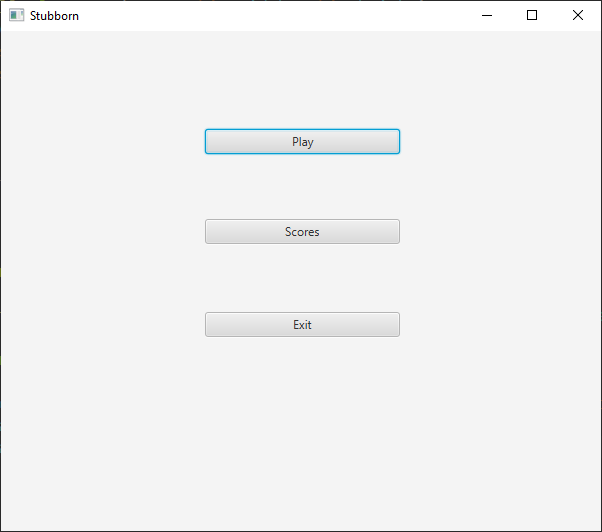
\includegraphics[width=\textwidth,height=\textheight,keepaspectratio]{img/menu.png}
\caption{Schermata di menu}
\label{img:menu}
\end{figure}
Se si preme su \textbf{Play} la partita inizia immediatamente, come si puo' notare dallo screenshot sottostante il quadratino verde indica il \textbf{player}, mentre i quadratini gialli e grigi sono rispettivamente gli \textbf{oggetti collezionabili} e i \textbf{nemici}. Si hanno a disposizione 3 vite, quando si arriva a 0 la partita termina e si ritorna al menu di gioco, quindi si ha la possibilita' di iniziarne una nuova.
\begin{figure}[H]
\centering{}
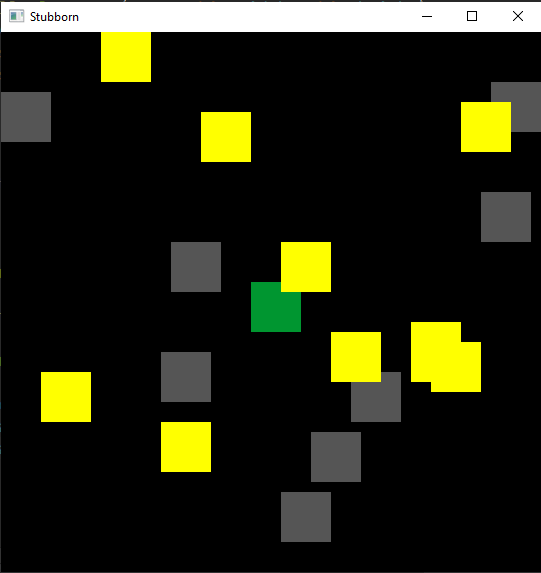
\includegraphics[width=\textwidth,height=\textheight,keepaspectratio]{img/game.png}
\caption{Schermata di gioco}
\label{img:game}
\end{figure}
\bibliography{report}
\begin{itemize}
    \item MVP: Model-View-Presenter The Taligent Programming Model for C++ and Java (document) 
    \item Design Patterns doc e tutorial \url{https://refactoring.guru/design-patterns}
    \item JavaFx documentation \url{https://openjfx.io/}  
    \item JavaFx repository \url{https://github.com/openjdk/jfx}
\end{itemize}
\end{document}
